\section{Clases modificadas}\label{ModificClass}

\setbeamercolor{block title}{bg=blue!50!black,fg=white}
\setbeamercolor{block body}{bg=blue!20,fg=white}

\begin{frame}
    \begin{columns}[t]
        \begin{column}{.5\textwidth}
          \tableofcontents[sections={1-2},currentsection]
        \end{column}
        \begin{column}{.5\textwidth}
          \tableofcontents[sections={3-4},currentsection]
        \end{column}
    \end{columns}
\end{frame}

\subsection{Moogle.cs}
 

\begin{frame}[fragile]{Moogle.cs}

    \only<1>{\textbf{Moogle.cs}\\
    Principal clase, en la cual se cablean todos los métodos implementados para trabajar la query y asegurar así
    una respuesta al usuario.}

    
    \only<1>{\begin{figure}[h]
        \center
        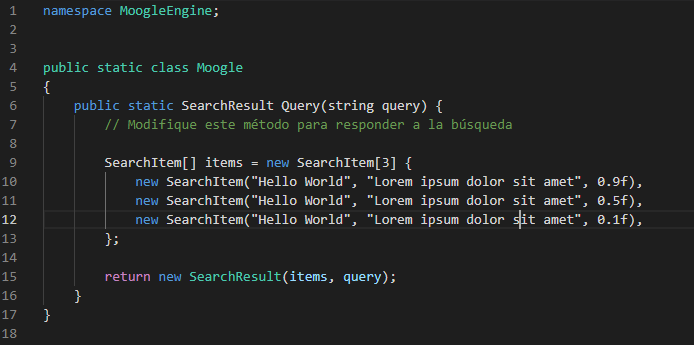
\includegraphics[width=8cm]{moogle1.jpg}
        \caption{Código que presentaba dicha clase al inicio}
     \end{figure}}

    \only<2>{\begin{figure}[h]
        \center
        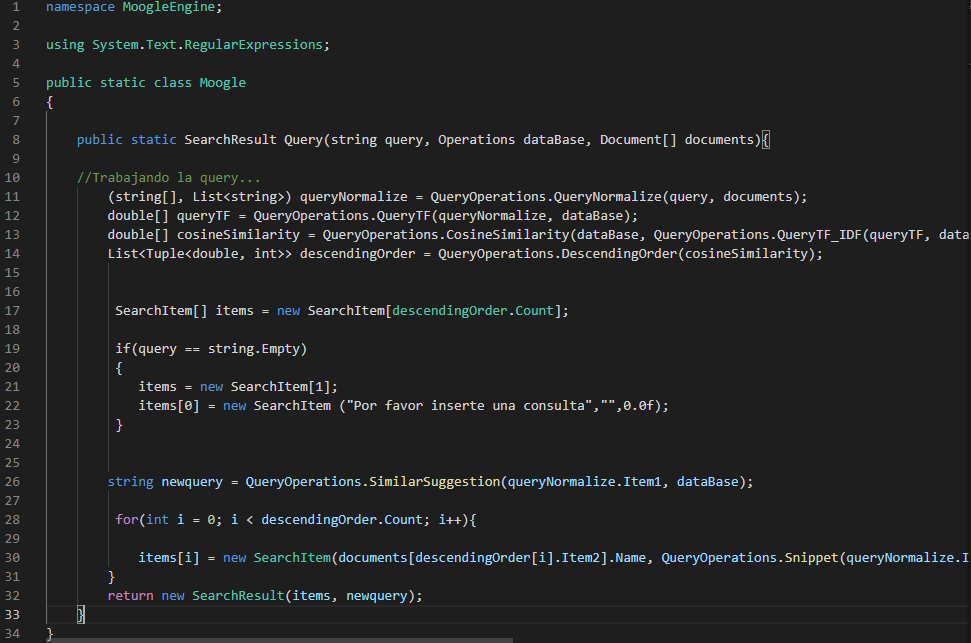
\includegraphics[width=8cm]{moogle2.jpg}
        \caption{Código que presenta actualmente}
     \end{figure}}

\end{frame}

\subsection{Program.cs}

\begin{frame}[fragile]{Program.cs}

    \only<1>{\textbf{Program.cs}\\
    Clase encargada de hacer que sean normalizados y pre-calculados los valores de cada documento que tengamos 
    como base de datos.}


    \only<2>{\begin{figure}[h]
        \center
        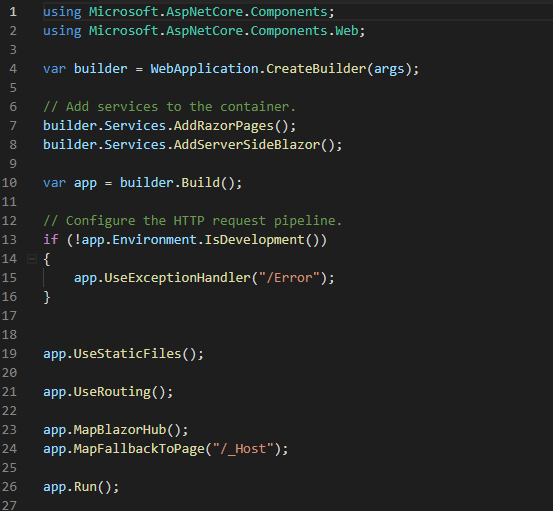
\includegraphics[width=6cm]{program1.jpg}
        \caption{Código que presentaba dicha clase al inicio}
     \end{figure}}

    \only<3>{\begin{figure}[h]
        \center
        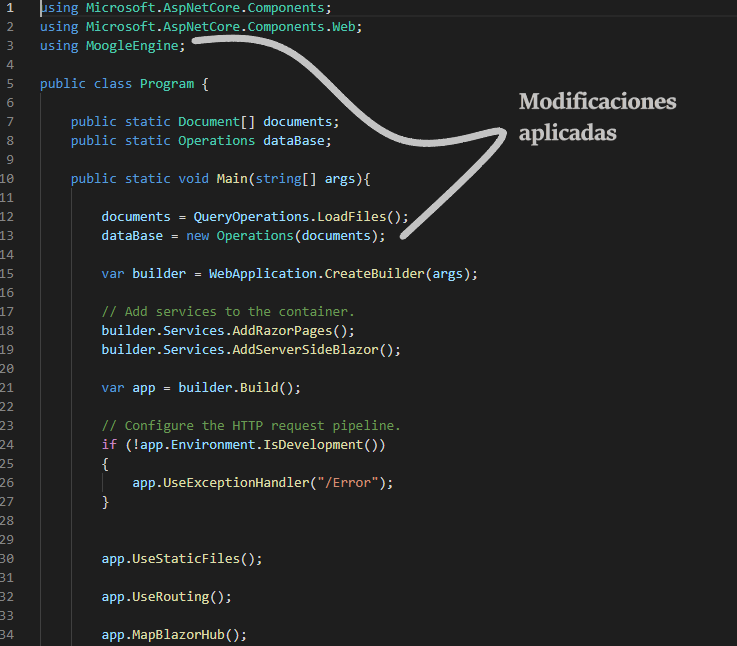
\includegraphics[width=7cm]{program2m.jpg}
        \caption{Código que presenta actualmente}
     \end{figure}}

\end{frame}

\subsection{Index.razor}

\begin{frame}[fragile]{Index.razor}

    \only<1>{\textbf{Index.razor}\\
    Clase en la que se desarrollan los comando que formarán la interfaz gráfica del proyecto.}

    \only<2>{\begin{figure}[h]
        \center
        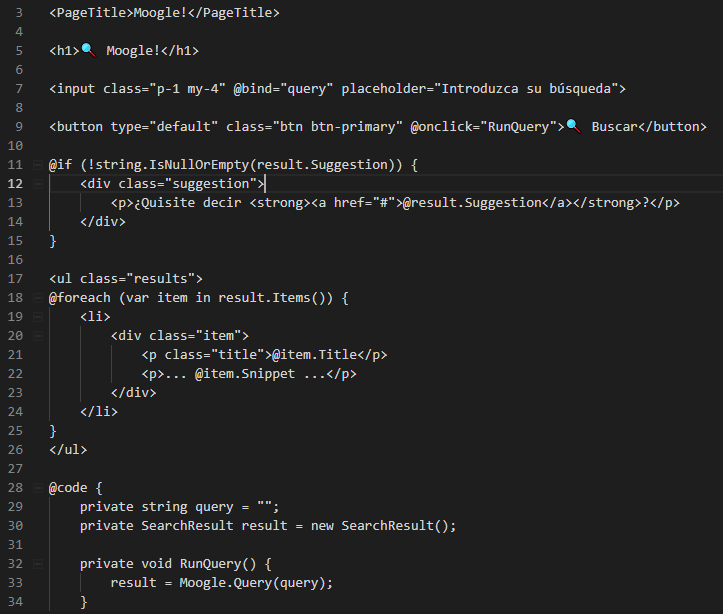
\includegraphics[width=7cm]{index_razor1.jpg}
        \caption{Código que presentaba dicha clase al inicio}
     \end{figure}}

     \only<3>{\begin{figure}[h]
        \center
        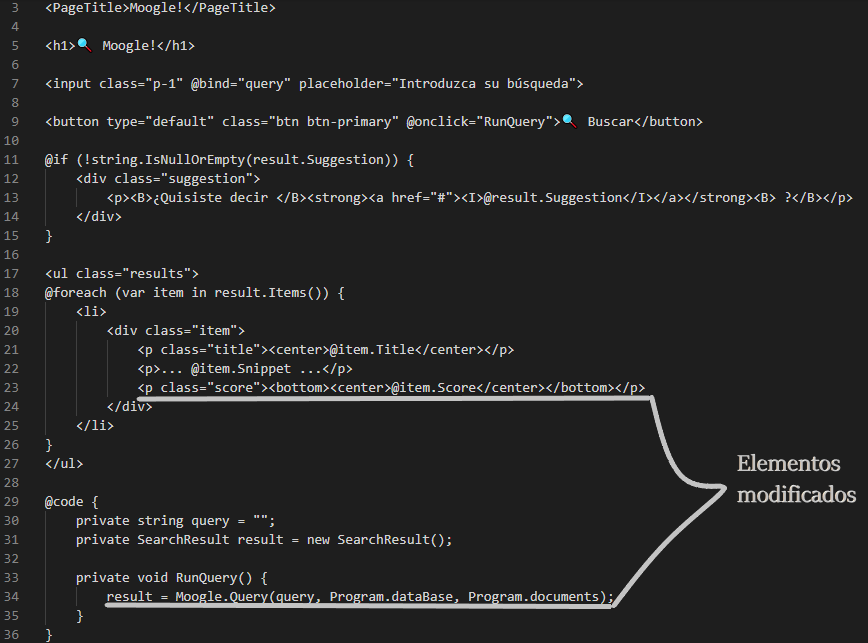
\includegraphics[width=7cm]{index_razor2m.jpg}
        \caption{Código que presenta actualmente}
     \end{figure}}

\end{frame}

\subsection{Index.razor.css}

\begin{frame}[fragile]{Index.razor.css}

    \only<1>{\textbf{Index.razor.css}\\
    Clase en la cual se desenvuelve el diseño que tendrá la interfaz gráfica aplicando colores, fuentes
    de letras, tamaños y formas a las distintas partes que la conforman.}

    \only<1>{\begin{figure}[h]
        \center
        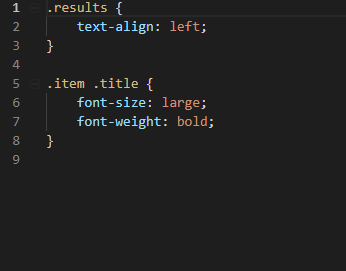
\includegraphics[width=5cm]{index_css1.jpg}
        \caption{Código que presentaba dicha clase al inicio}
     \end{figure}}

     \only<2>{\begin{figure}[h]
        \center
        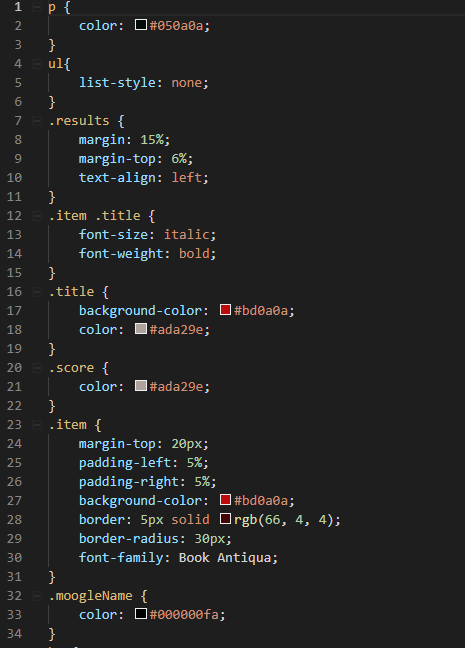
\includegraphics[width=4cm]{index_css2.jpg}
        \caption{Código que presenta actualmente}
     \end{figure}}
    
\end{frame}
